\documentclass[11pt,a4paper]{article}
\usepackage[margin=2.25cm]{geometry}
\usepackage{setspace}
\setstretch{1.08}
\usepackage{amsmath,amssymb}
\usepackage{booktabs}
\usepackage{siunitx}
\usepackage{tikz}
\usetikzlibrary{arrows.meta,positioning}
\usepackage{graphicx}
\usepackage[hidelinks]{hyperref}

\title{Compliance-Aware Vision Metering\\for a Wooden Seed-Planting Row Unit}
\author{System Design Study\\[0.3em]
\large Short paper on the first innovation of the wooden seed-planter thesis}
\date{}

\begin{document}
\maketitle

\begin{abstract}
Irregular woody seed singulates poorly on a cell plate, and a laminated-timber row unit moves while the seed is falling. A vision loop that treats every late seed as an empty cell will advance the plate too often and create the doubles it was meant to prevent. This paper specifies a per-row controller that labels cells, estimates boot motion with a model of the timber flexure, and repairs an empty cell only when the repair can finish before the gate. Mean depth is assigned to a servo slower than the arm resonance. Resonant speeds are excluded rather than cancelled. On the design model the repair holds the quality-of-feed index near \(0.98\) from \(0.8\) to \(1.8\,\mathrm{m/s}\) and withdraws as the hole period approaches the sensing delay.
\end{abstract}

\noindent\textbf{Keywords:} seed metering, machine vision, wooden planter, Kalman filter, depth control.

\section{Introduction}
A precision meter is supposed to release one seed each time a cell passes the gate. The agronomic object is the spacing in the furrow. The engineering substitute is the set of spacings classified against a target \(x_{\mathrm{ref}}\): a spacing below half the target is a multiple, a spacing above one and a half times the target is a miss, and the rest are singles \cite{iso7256,kachman1995}. The quality-of-feed index is the frequency of singles. A single coefficient of variation over every spacing mixes skips with scatter, so the miss and multiple indices are kept separate \cite{kachman1995}.

Woody and native seed makes the classification harder. The seed is irregular, the depth band is narrow, and many practical tools are still hand jabs or hollow tubes \cite{usdaplanter,masarei2019}. A timber row unit is attractive because it can be laminated locally and because wood dissipates vibration. The same compliance moves the boot. Soil force of a few tens of newtons on a link sized for a light machine deflects the release gate by millimetres, and a seed that is still in view because the gate moved looks like a miss.

Published vision loops already show both halves of the problem. A camera on a pneumatic maize meter cut missed hills at \(2\) and \(4\,\mathrm{km/h}\) and increased them at \(6\,\mathrm{km/h}\), because the detector was right and the processor was late \cite{borja2018,borja2021}. Detectors of the YOLO family now name empty cells and doubles at errors of about two percent on peanut and maize meters \cite{blaser2024,zhao2025yolo}. High-speed imaging of an electric-drive meter held singulation near \(98\%\) across a wide speed range and lost it when the machine accelerated or when the seed rate rose \cite{mangus2017}. None of those results writes a timber flexure into the decision to repair.

This paper specifies that decision. The controller is the metering half of a four-row wooden planter. It does not choose the vehicle heading. It publishes the speeds at which a repair is still timely and at which the arm magnification stays bounded. A coverage controller may use that set. It may not keep a private speed of its own.

\section{Flexure and seed flight}
The boot displacement \(\delta\), positive downward, is one equivalent mass on a timber stiffness,
\begin{equation}
\label{eq:arm}
m_{\mathrm{eq}}\ddot{\delta}+c_d\dot{\delta}+k\delta=F_{\mathrm{soil}}+F_{\mathrm{act}},
\end{equation}
with \(c_d=2\zeta\sqrt{km_{\mathrm{eq}}}\). The design values are \(k=8200\,\mathrm{N/m}\), \(m_{\mathrm{eq}}=6.8\,\mathrm{kg}\) and \(\zeta=0.08\), so the undamped frequency is \(f_n=5.53\,\mathrm{Hz}\) and a static soil force of \(80\,\mathrm{N}\) deflects the boot by \(9.8\,\mathrm{mm}\). That offset is already outside an \(\pm 8\,\mathrm{mm}\) band around an \(18\,\mathrm{mm}\) target if nobody removes it.

Roughness of wavelength \(\lambda\) met at speed \(v\) arrives at frequency \(v/\lambda\). The dynamic magnification of a viscously damped oscillator grows as that frequency approaches \(f_n\). With a \(30\,\mathrm{N}\) roughness component at \(\lambda=0.45\,\mathrm{m}\), the disturbance frequency at \(2.4\,\mathrm{m/s}\) is \(5.33\,\mathrm{Hz}\) and the magnification is near \(6\). A depth servo is not asked to cancel that peak. The peak is a speed the machine is not allowed to hold.

After release, a seed dropped through \(H=0.42\,\mathrm{m}\) is in the air for about \(0.29\,\mathrm{s}\). The machine travels \(v\) times that flight, about \(0.41\,\mathrm{m}\) at \(1.4\,\mathrm{m/s}\), which is two target spacings of \(0.20\,\mathrm{m}\). The tube is built to cancel the mean of that transport. It cannot cancel a gate velocity that changes from seed to seed. An arm velocity of \(0.04\,\mathrm{m/s}\) shifts the landing by about \(12\,\mathrm{mm}\). The filter therefore carries exit velocity so the seed map records the shift instead of blaming the plate.

Vacuum, if the plate is pneumatic, is sized with the vibration acceleration included, following the dependence of holding pressure on seed mass, orifice area and plate acceleration \cite{karayel2004}. The nominal pressure is not modulated inside one hole period. A wooden hopper does not contain a plenum that settles that fast. A slow trim may lower pressure only when logged doubles exceed logged misses over ten metres.

\section{What the camera is allowed to change}
The continuous state on one row is boot displacement and velocity, a depth bias, the time until the next release, and the horizontal exit velocity. The cell label, empty or single or double, sits beside that state. It is not a sixth continuous coordinate. Between frames the release time counts down. Arm velocity shifts the predicted release, because a moving lip crosses the seed earlier or later than a rigid schedule. Only the delay that remains after that shift is offered to the miss logic.

The images are fused with boot force, an ultrasonic range and an inertial measurement in an unscented Kalman filter \cite{julier1997,sarkka2013}. Process noise on the boot grows with the magnification, so a resonant arm is not treated as a calm mechanism. A low-confidence frame widens the release-time noise and does not authorise a repair. A dropped frame is handled the same way. Extending the vision budget to finish a late frame is the failure mode already measured on a slow processor \cite{borja2021}.

The plate command is the feedforward that matches \(N=24\) cells to ground speed and spacing, plus three corrections. A small trim advances or retards an occupied cell whose predicted release has drifted, and it is saturated at eight percent of the feedforward. A double reduces plate speed for one hole period and does not pretend the extra seed can be called back. An empty cell is replaced by a one-pitch advance only when the repair fraction is high. That fraction is \(1\) when the hole period \(x_{\mathrm{ref}}/v\) clears the sum of vision and actuator delay, \(57\,\mathrm{ms}\) in the design, with a margin and a surcharge for acceleration. It falls toward a floor of \(0.15\) when the period does not clear that test. The floor is a refusal, not a random repair. The feasible speed set reported upward is the set where the repair fraction at zero acceleration is at least \(0.85\), with the resonant neighbourhood removed. On the design spacing that latency cut lies near \(1.87\,\mathrm{m/s}\).

\begin{figure}[t]
\centering
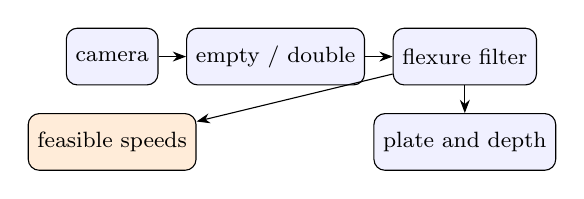
\begin{tikzpicture}[font=\footnotesize, node distance=0.35cm, >=Stealth,
  box/.style={draw, rounded corners, align=center, minimum height=0.72cm, fill=blue!6}]
  \node[box] (cam) {camera};
  \node[box, right=of cam] (det) {empty / double};
  \node[box, right=of det] (ukf) {flexure filter};
  \node[box, below=of ukf] (law) {plate and depth};
  \node[box, fill=orange!15, below=of cam] (set) {feasible speeds};
  \draw[->] (cam) -- (det);
  \draw[->] (det) -- (ukf);
  \draw[->] (ukf) -- (law);
  \draw[->] (ukf) -- (set);
\end{tikzpicture}
\caption{Per-row metering. The vehicle receives a feasible speed set, not a plate command.}
\label{fig:loop}
\end{figure}

Depth uses a proportional-integral force on the filtered boot error and a rate term that adds to wood damping. The target bandwidth is \(3\,\mathrm{Hz}\), below \(f_n\). The integral is frozen when the boot is lifted or when the ultrasonic innovation is rejected. Actuator force is saturated at \(120\,\mathrm{N}\). The split is deliberate. The servo removes the mean deflection. Vehicle speed keeps the roughness frequency away from resonance. A loop fast enough to cancel the peak would need a bandwidth the timber link is not asked to provide.

Four rows are four copies of this filter. They share the vehicle clock and the ground speed. Each detector thread has a reserved budget of \(22\,\mathrm{ms}\) inside the \(57\,\mathrm{ms}\) delay. A frame that misses the deadline is cancelled. Realised delay, measured from the exposure stamp to the stepper command, tightens the repair fraction if the hardware is slower than the specification. A fast swath does not loosen it on the same day.

\section{Modelled indices}
The map used to score speeds is explicit, so a planner can evaluate it without resimulating every seed. Open-loop misses rise with speed, with acceleration, and with the dynamic boot amplitude. Closed-loop misses apply the repair fraction, a recall of \(0.99\) and a further small loss, plus a floor for false repairs. Doubles are reduced only in part. Depth error keeps a bias the open loop does not remove and credits the servo with rejection only while the roughness frequency stays near or below \(3\,\mathrm{Hz}\). These expressions are estimation devices placed in the qualitative range of the metering literature. They are not a woody-seed trial. Detector scores taken from peanut and maize are an upper bound for a more irregular seed \cite{blaser2024,zhao2025yolo}.

\begin{table}[t]
\centering
\caption{Modelled index at zero acceleration.}
\label{tab:qfi}
\begin{tabular}{@{}rrrrr@{}}
\toprule
\(v\) & \(c\) & \(\mathrm{QFI}_{ol}\) & \(\mathrm{QFI}_{cl}\) & \(\sigma_z\) \\
(m/s) & & & & (mm) \\
\midrule
1.0 & 1.00 & 0.881 & 0.981 & 1.79 \\
1.4 & 1.00 & 0.834 & 0.978 & 2.14 \\
1.8 & 1.00 & 0.781 & 0.974 & 3.52 \\
2.0 & 0.80 & 0.750 & 0.927 & 5.00 \\
2.4 & 0.33 & 0.653 & 0.752 & 13.20 \\
\bottomrule
\end{tabular}
\end{table}

Table~\ref{tab:qfi} is that map at zero acceleration. From \(1.0\) to \(1.8\,\mathrm{m/s}\) the closed-loop index stays on a plateau near \(0.98\) while the open-loop index falls from \(0.88\) to \(0.78\). Depth error grows from \(1.8\) to \(3.5\,\mathrm{mm}\) and is still inside a \(4\,\mathrm{mm}\) design ceiling at \(1.8\,\mathrm{m/s}\). At \(2.0\,\mathrm{m/s}\) the repair fraction drops, the index falls to \(0.93\), and depth error reaches \(5\,\mathrm{mm}\). At \(2.4\,\mathrm{m/s}\) the closed loop still beats the open loop and still fails the band, which is why resonance is excluded instead of being left to the servo. At fixed \(1.8\,\mathrm{m/s}\), accelerations of \(0\), \(0.4\), \(0.8\) and \(1.2\,\mathrm{m/s}^2\) give repair fractions \(1.00\), \(0.98\), \(0.85\) and \(0.71\). A headland brake near \(0.7\,\mathrm{m/s}^2\) remains on the safe side of that test at the speeds where repairs are otherwise allowed.

One empty cell at \(1.4\,\mathrm{m/s}\) shows the arithmetic. The hole period is \(0.143\,\mathrm{s}\) and the feedforward plate speed is \(1.83\,\mathrm{rad/s}\). The repair test is satisfied. If \(68\,\mathrm{ms}\) remain after inference, a one-pitch advance fits inside the \(35\,\mathrm{ms}\) actuator budget. The same test at \(2.2\,\mathrm{m/s}\) withholds the advance. The empty cell is logged as a miss and is not filled late.

\section{Timing budget and the repairs that are refused}
The loop is not one clock. The camera runs at \(30\,\mathrm{Hz}\), which at \(1.5\,\mathrm{m/s}\) and a \(0.20\,\mathrm{m}\) spacing gives several frames of each cell before the gate. The filter runs at \(100\,\mathrm{Hz}\) so a release can be stamped more finely than a frame. The depth screw is updated at \(50\,\mathrm{Hz}\) inside the \(3\,\mathrm{Hz}\) bandwidth. The feasible-speed message goes out at \(10\,\mathrm{Hz}\). Exposure and readout are allocated \(8\,\mathrm{ms}\) of the vision delay, inference \(14\,\mathrm{ms}\), and the stepper \(35\,\mathrm{ms}\). Those allocations are the delay the repair test uses. A build that misses an allocation must shrink the feasible set. It must not keep the test and hope.

Three situations look like chances to be clever and are refused. An empty hopper sector cannot be repaired by advancing the plate, so the advance is inhibited and the schedule is left alone. If the measured delay from exposure to the stepper command exceeds the budget for three holes, repairs stop even if the specification still says they fit. Vacuum is not raised in the same hole as plate speed. Each action can cut misses, and stacking them is how a correct detector manufactures doubles. One action per hole, and no action when the repair fraction is low, is the rule.

A planting day starts with one calibration swath, plates disengaged, boot in the soil, at three depth set-points. The slope of boot force against depth is the local soil stiffness. The intercept is the static force the servo must remove. If that force is \(110\,\mathrm{N}\) rather than \(80\,\mathrm{N}\), the undeflected offset is \(13.4\,\mathrm{mm}\) instead of \(9.8\,\mathrm{mm}\), still inside the screw travel, and the integral term works harder. The same pass can replace the design roughness wavelength. A wavelength of \(0.30\,\mathrm{m}\) moves the resonant speed from about \(2.4\,\mathrm{m/s}\) to about \(1.7\,\mathrm{m/s}\), inside the range the latency test would otherwise allow. The feasible set then has a hole, and steady running stays on the quiet side of it. A saturated force signal, which yields no intercept, inhibits planting. Running the workshop numbers against an unmeasured soil is the alternative the interlock refuses.

The seed map stores two stamps. The vehicle pose when the detector fires and the estimated landing after the \(0.29\,\mathrm{s}\) flight differ by about \(0.41\,\mathrm{m}\) at \(1.4\,\mathrm{m/s}\), which is two target spacings. A later survival count joined to the wrong stamp would teach the next cost to fear the wrong places. Logged delay may tighten the repair test on the next swath. A swath that happens to be fast does not loosen the test on the same day. Adaptation that only tightens cannot talk the machine into the late-repair regime.

\section{Where this controller stops}
This design publishes a set of speeds. It does not steer, and it does not pick a heading. The plate law uses the ground speed the vehicle actually has. If slip on a grade drops that speed, the plate slows with it and the spacing holds. If a plan sent the intended speed while the wheels were still slow, seeds would bunch at the start of every swath. The index plateau in Table~\ref{tab:qfi} is the region a coverage search is allowed to use. Spending the last tenth of a metre per second before the cliff buys almost no singulation change and, on the work model of the companion paper, almost no energy change. Crossing the cliff does. The hard set is how that cliff is kept out of the plan.

The same formulas score a shorter prescription. At \(0.12\,\mathrm{m}\) spacing and \(1.4\,\mathrm{m/s}\) the hole period falls from \(0.143\,\mathrm{s}\) to \(0.086\,\mathrm{s}\), below the repair threshold, and the admissible speed falls to about \(1.1\,\mathrm{m/s}\). The metering law does not discover that violation by attempting late repairs. The feasible set moves with the local spacing before the vehicle is asked to hold \(1.4\,\mathrm{m/s}\) on a dense patch.

What remains empirical is the detector on this seed and this wooden tube. The recall used in the closed-loop map is taken from peanut and maize results. A woody seed is a harder object, and a brown tube is a harder background. If a belt test at \(1.4\,\mathrm{m/s}\) with a healthy delay returns a quality-of-feed index of \(0.90\) rather than \(0.98\), the map was optimistic and the number is retired. The speed test, the depth split, and the refusal to repair late would remain, because none of them is the recall figure.

\section{Conclusion}
Compliance-aware vision metering repairs an empty cell only while the hole period still contains the sensing and actuation delay, and it explains part of a late image by the motion of the timber arm before it declares a miss. Mean depth is servoed below the arm's natural frequency. Resonant running is refused. On the design model the resulting index plateau sits near \(0.98\) up to \(1.8\,\mathrm{m/s}\) and ends when either the delay or the resonance binds. The numbers are model scores under published detector performance. A belt test with the woody seed, and a second camera the controller does not see, is what would replace them.

\begin{thebibliography}{12}
\bibitem{iso7256}
ISO, ``Sowing equipment---Test methods---Part 1: Single seed drills,'' ISO 7256-1, 1984.
\bibitem{kachman1995}
S.~D. Kachman and J.~A. Smith, ``Alternative measures of accuracy in plant spacing for planters using single seed metering,'' \emph{Trans. ASAE}, vol.~38, no.~2, pp.~379--387, 1995.
\bibitem{usdaplanter}
USDA Forest Service, ``Evaluation of single-seed planters,'' Tech Tip 1024-2306P-MTDC.
\bibitem{masarei2019}
M.~Masarei, A.~L. Guzzomi, D.~J. Merritt, and T.~E. Erickson, ``Improvements to mechanical direct seeder design guided by the optimal sowing depth of soft spinifex,'' in \emph{Mine Closure}, 2019.
\bibitem{borja2018}
A.~A. Borja, R.~M.~C. Amongo, D.~C. Suministrado, and J.~P. Pabico, ``A machine vision assisted mechatronic seed meter for precision planting of corn,'' in \emph{ICCRE}, 2018, pp.~183--187.
\bibitem{borja2021}
A.~A. Borja, R.~M. Amongo, D.~C. Suministrado, and J.~P. Pabico, ``Design and evaluation of a machine vision system and mechatronic drive for a pneumatic seed meter for corn,'' \emph{Philipp. J. Agric. Biosyst. Eng.}, 2021.
\bibitem{blaser2024}
M.~Blaser, W.~Porter, L.~Fuhrer, and T.~Bourlai, ``YOLOv10 computer vision performance measurement for agricultural vacuum seed meters,'' in \emph{IEEE BigData}, 2024, pp.~1929--1936.
\bibitem{zhao2025yolo}
P.~Zhao \emph{et al.}, ``Performance evaluation of a high-speed maize seed-metering device using an improved YOLOv5s,'' \emph{Smart Agric. Technol.}, vol.~11, 100997, 2025.
\bibitem{mangus2017}
D.~L. Mangus \emph{et al.}, ``Development of high-speed camera hardware and software to evaluate real-time electric seed meter accuracy,'' \emph{Comput. Electron. Agric.}, vol.~142, pp.~314--325, 2017.
\bibitem{karayel2004}
D.~Karayel, Z.~B. Barut, and A.~\"Ozmerzi, ``Mathematical modelling of vacuum pressure on a precision seeder,'' \emph{Biosyst. Eng.}, vol.~87, no.~4, pp.~437--444, 2004.
\bibitem{julier1997}
S.~J. Julier and J.~K. Uhlmann, ``A new extension of the Kalman filter to nonlinear systems,'' in \emph{AeroSense}, 1997.
\bibitem{sarkka2013}
S.~S\"arkk\"a, \emph{Bayesian Filtering and Smoothing}. Cambridge Univ. Press, 2013.
\end{thebibliography}

\end{document}
